%%%%%%%%%%%%%%%%%%%%%%%%%%%%%%%%%%%%%%%%%%%%%%%%%%%
%
%  New template code for TAMU Theses and Dissertations starting Fall 2016.
%
%  Author: Sean Zachary Roberson
%	 Version 3.16.09
%  Last updated 9/12/2016
%
%%%%%%%%%%%%%%%%%%%%%%%%%%%%%%%%%%%%%%%%%%%%%%%%%%%
%%%%%%%%%%%%%%%%%%%%%%%%%%%%%%%%%%%%%%%%%%%%%%%%%%%%%%%%%%%%%%%%%%%%%%
%%                           SECTION III
%%%%%%%%%%%%%%%%%%%%%%%%%%%%%%%%%%%%%%%%%%%%%%%%%%%%%%%%%%%%%%%%%%%%%



\chapter{KINETICS EXAMPLES}\label{sect:kin}

Neutron dynamics is the study of the time-dependent nature of neutrons in a reactor.  More specifically, there is no coupling of neutron behavior with other physics, like thermal hydraulic feedback.  This section describes kinetics examples that IQS is tested with and analysis of its performance.  The examples range in complexity and application.  The first is a one-dimensional problem, designed for the prototype code in MATLAB.  The next four are from the Argonne National Lab (ANL) Benchmark Problem Book (BPB), and are common problems for testing codes and developing methods \cite{ANL_BPB}. 

\section{One Dimensional Prototype Problem}

This example is very simple and computes quickly; it entails a one dimensional, homogeneous 400 cm slab with a heterogenous perturbation in absorption cross section.  \fig{fig:slab} shows how the regions of the slab are divided and \tbl{tab:1Dmat} shows the initial material properties.  Regions 2, 3, and 4 have slope perturbations at different points in time, \tbl{tab:1Dslope} shows the values of the absorption cross-section in each region at the times of interest.  The values of $\Sigma_a$ between these times of interest are linear interpolations between the given values.

\begin{figure}[!htbp]
\begin{center}
\begin{tabular}{| l | l | l | l | l | l | l | l | l | l | l | l | l | l | l | l | l | l | l | l |}
\hline \hline \hline
  &   &   &   &   &   &    &    &   &   &   &   &   &   &   &   &   &   &   &   \\
1 & 1 & 1 & 1 & 2 & 3 & 1 & 1 & 1 & 1 & 1 & 1 & 1 & 1 & 4 & 4 & 1 & 1 & 1 & 1 \\
  &   &   &   &   &   &    &    &   &   &   &   &   &   &   &   &   &   &   &   \\
\hline \hline \hline
\end{tabular}
\caption{1-D slab region identification}
\label{fig:slab}
\end{center}
\end{figure}

\begin{table}[!htbp]
\begin{center}
\caption{1-D slab material properties and problem parameters}
\label{tab:1Dmat}
\begin{tabular}{llllll}
\hline
$D (cm)$ & $\Sigma_a (cm^{-1})$ & $\nu \Sigma_f (cm^{-1})$ & $v (cm/s)$ & $\beta$ & $\lambda (s^{-1})$ \\
\hline
1.0 & 1.1 & 1.1 & 1,000 & 0.006 & 0.1 \\

\hline
\end{tabular}
\end{center}
\end{table}

\begin{table}[!htbp]
\begin{center}
\caption{1-D slab absorption cross-section at times of interest}
\label{tab:1Dslope}
\begin{tabular}{llllllll}
\hline
Region & Material Property & 0.0 s & 0.1 s & 0.6 s & 1.0 s & 1.7 s \\
\hline
2 & $\Sigma_{a} (cm^{-1})$ & 1.1 & 1.1 & 1.095 & 1.095 & 1.095 \\
3 & $\Sigma_{a} (cm^{-1})$ & 1.1 & 1.1 & 1.09 & 1.09 & 1.1 \\
4 & $\Sigma_{a} (cm^{-1})$ & 1.1 & 1.1 & 1.105 & 1.105 & 1.105 \\
\hline
\end{tabular}
\end{center}
\end{table}

\fig{fig:1D_power} shows the resulting baseline relative power profile of the one-dimensional problem.  The baseline was computed using MATLAB's ode15s function which is a embedded Runge-Kutta time adaptive method for stiff problems, the error tolerance was set very tightly ($10^{-12}$).  This baseline computation is used to compute the error of the other time discretization methods.  \fig{fig:1D_shape} shows the shape profile at various times during the transient.  It is apparent that the shape is very time-dependent, so it is expected that IQS has marginal accuracy gain for a given time step.

\begin{figure}[!htbp]
\begin{center}
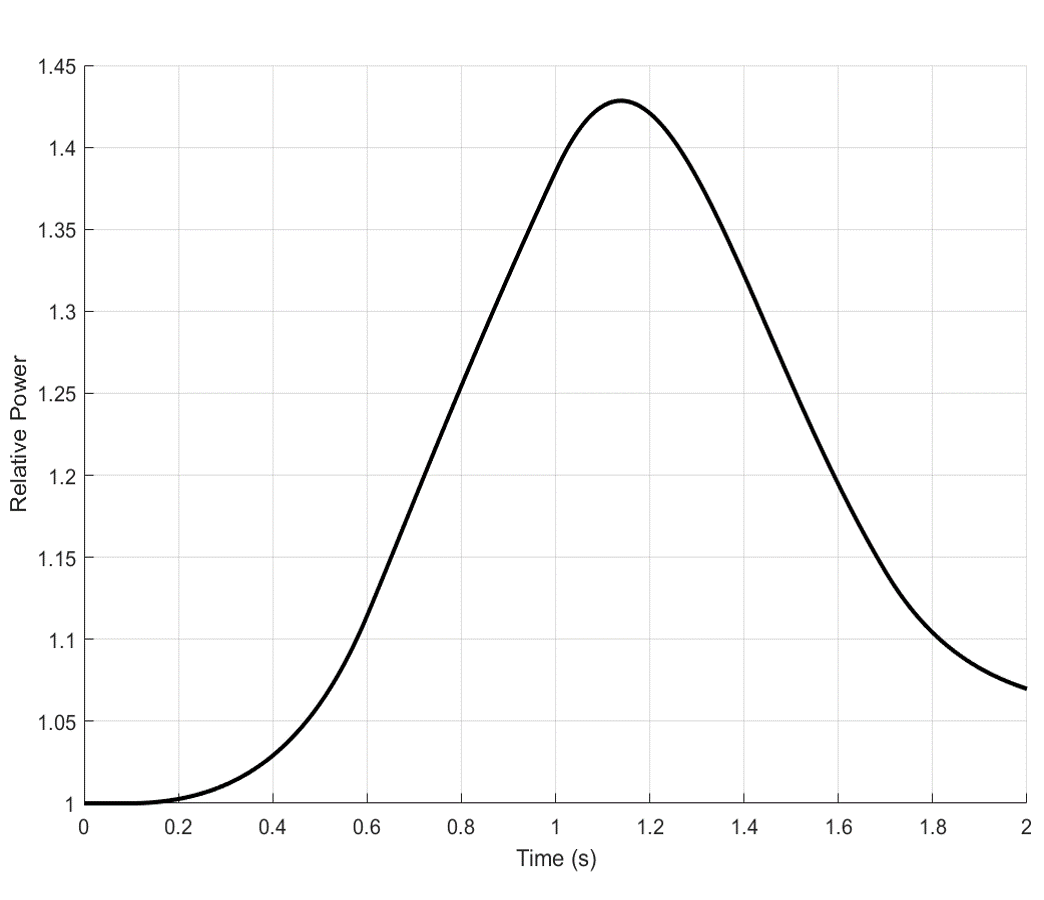
\includegraphics[width=\linewidth]{\FiguresDir/1D_power_base.png}
\caption{Baseline total power level for the 1D slab test case}
\label{fig:1D_power}
\end{center}
\end{figure}

\begin{figure}[!htbp]
\begin{center}
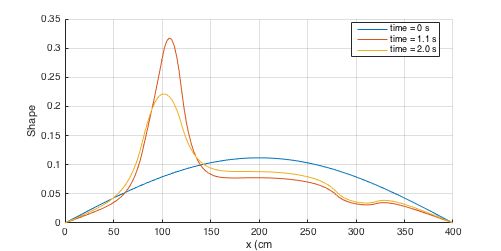
\includegraphics[width=\linewidth]{\FiguresDir/1D_shape.png}
\caption{Flux profile of 1D slab at various times}
\label{fig:1D_shape}
\end{center}
\end{figure}

\subsection{IQS Iteration Convergence}

IQS, as previously stated, is a system of nonlinear equations between shape and amplitude. These equations needed to be iterated to numerically converge to an accurate solution.  \sct{sect:iter} describes various iteration techniques for fixed-point and Newton schemes. \fig{fig:iter} shows the number of fixed-point iterations required for a $10^{-11}$ tolerance over the transient. The criteria listed in the legend are described as:
\begin{enumerate}
\item $L^{\infty} \rightarrow$ \eqt{eq:shape_Linf}
\item $L^{2} \rightarrow$ \eqt{eq:shape_L2}
\item Reactivity $\rightarrow$ \eqt{eq:rho_conv}
\item Amplitude $\rightarrow$ \eqt{eq:p_conv}
\item K criteria $\rightarrow$ \eqt{eq:K_conv}
\item All properties $\rightarrow$ \eqtss{eq:rho_conv}{eq:K_conv}
\end{enumerate}
This plot shows that 1-4 have approximately the same convergence behavior, but the K criteria converges to a certain error. \fig{fig:iter_err} shows the resulting error the K criteria converges to for different points of rescaling the shape. The rescaling is described by \eqt{eq:shape_scale}. Rescaling shape more frequently helps the error.  However, rescaling every iteration is somewhat artificial because it does not consider changes spatially. Regardless, an error of $~10^{-5}$ is quite large and it is expected that the magnitude is due to the explicit treatment of precursors (\eqt{eq:dnp_theta}). Switching to an analytical elimination (\eqt{eq:dnp_an}) does not converge as well, but the error is much smaller, seen in \fig{fig:iter_err_an}.

\begin{figure}[!htbp]
\centering
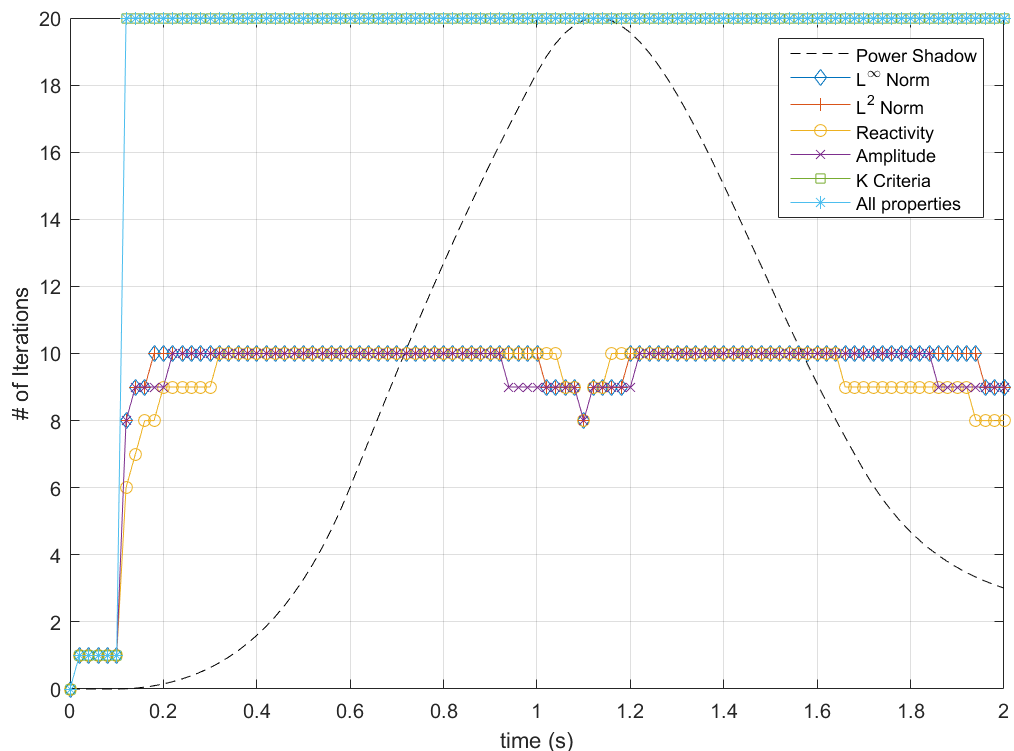
\includegraphics[width=0.75\linewidth]{\FiguresDir/iter_renorm.png}
\caption{\# of iterations for various convergence criteria, tolerance$=10^{-11}$, max iterations$=20$}
\label{fig:iter}
\end{figure}

\begin{figure}[!htbp]
\centering
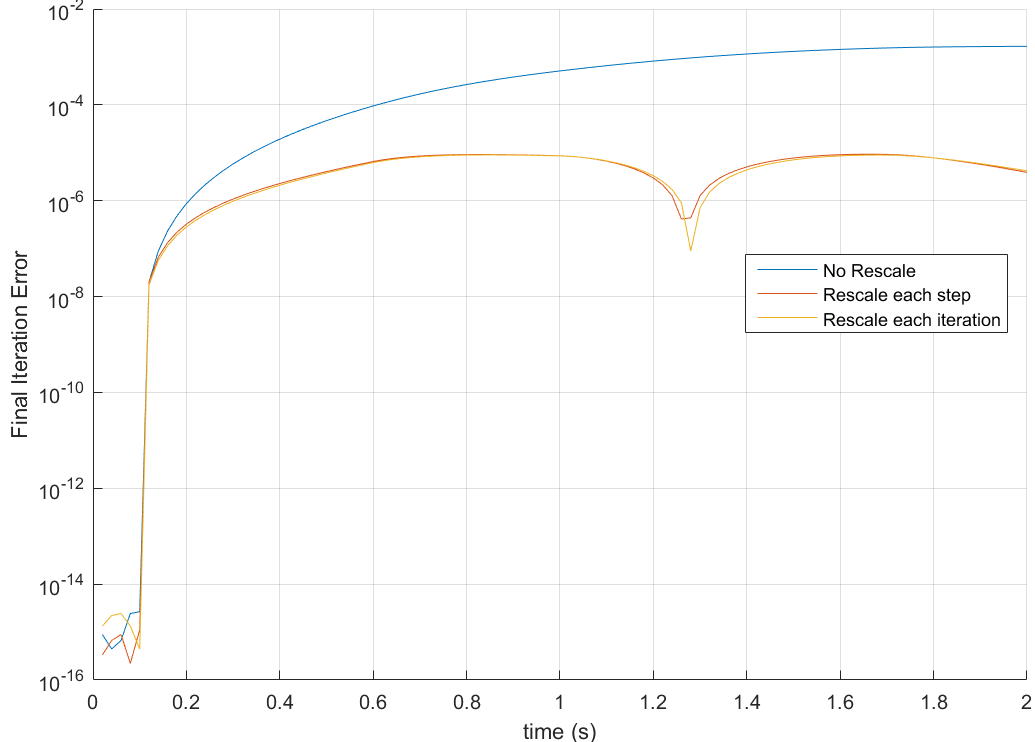
\includegraphics[width=0.75\linewidth]{\FiguresDir/iter_error.png}
\caption{Final iteration error for K convergence criteria}
\label{fig:iter_err}
\end{figure}

\begin{figure}[!htbp]
\centering
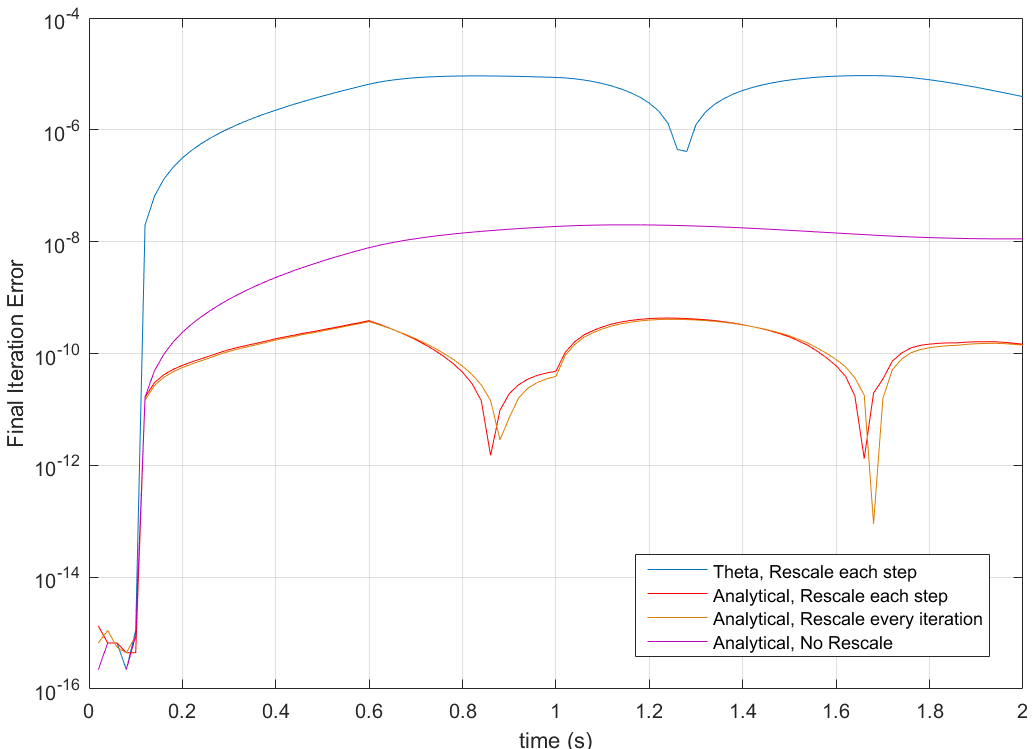
\includegraphics[width=0.75\linewidth]{\FiguresDir/iter_error_an.png}
\caption{Final iteration error for K convergence criteria with analytical precursor elimination}
\label{fig:iter_err_an}
\end{figure}


\subsection{Time Step Convergence}

Time step convergence analysis involves evaluating a problem with various refinements in step size and comparing the resulting errors with the time step size. Plotting error versus $\Delta t$ on a log-scale should produce a relatively strait line with a slope equal to the order of the time discretization method. In order to evaluate the performance and error convergence of IQS, the slab was simulated with varying time discretization methods and time step sizes.  \fig{fig:1D_conv} shows these convergence plots of five different discretization methods for implicit discretization, IQS, and IQS P-C.  These plots were generated from the results using the MATLAB prototype program.  The plots show that IQS and IQS P-C are convergent through fourth order BDF.  Third order SDIRK did not show third order convergence, but, through extensive testing, SDIRK shows non-convergent behavior for too stiff of problems.  

There are higher discretization order that can be tested, but most practical application do not go beyond second order.  This paper shows an analysis of the first publicized application of IQS with higher than second order discretization, which exposed unforeseen properties of IQS.  When using higher order techniques, the interpolation of PRKE parameters and shape for precursor integration become important to consider.  Every other application that was investigated linearly interpolates parameters for the PRKE evaluation.  Similarly, the shape used for the integration of the ODE for the precursors needs to have higher order interpolation to preserve high order error convergence.  This interpolation was done using Lagragian and Hermite methods, both leading to successful convergence.

The 1D slab problem was also applied to the Rattlesnake implementation of IQS.  \fig{fig:1D_conv_Rat} shows the error convergence for implicit Euler and BDF2 discretization of the three methods.  The results differ slightly from the prototype, especially in the fact that IQS P-C performs better than IQS.  Since Rattlesnake uses a PJFNK solver for the FEM model, number of time steps isn't strictly proportional to the execution time.  \fig{fig:1D_conv_lin} shows the error of the three methods as compared to the number of linear GMRES iterations, which is a better mark for comparison in computation time.  This figure shows that IQS performs worse than implicit discretization for most time-step sizes, but IQS P-C performs significantly better.  This is due to the fact that IQS needs to iterate between amplitude and shape to resolve its nonlinearity.

\begin{figure}[!htbp]
\centering
\begin{subfigure}[b]{0.49\textwidth}
\centering
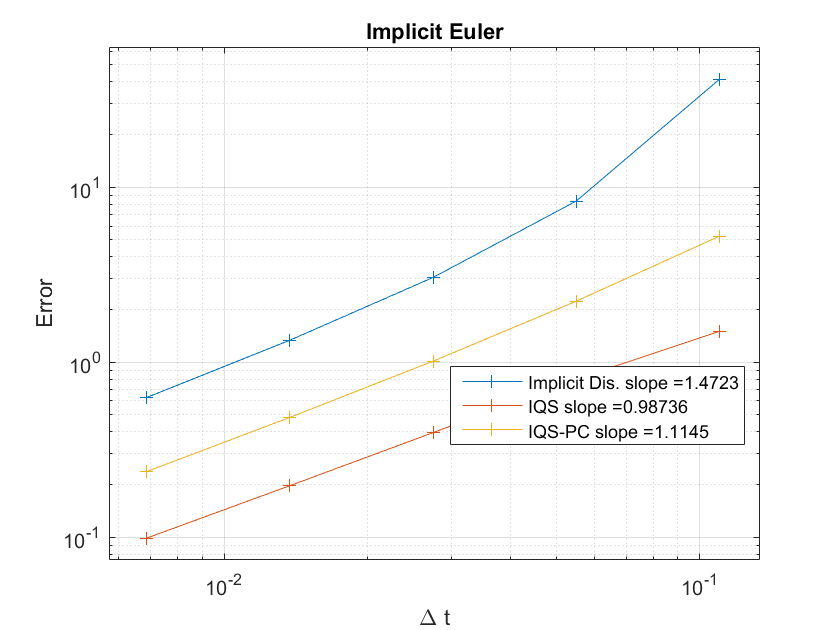
\includegraphics[width=\linewidth]{\FiguresDir/1D_conv_IE.png}
\caption{Implicit Euler}
\end{subfigure}
\begin{subfigure}[b]{0.49\textwidth}
\centering
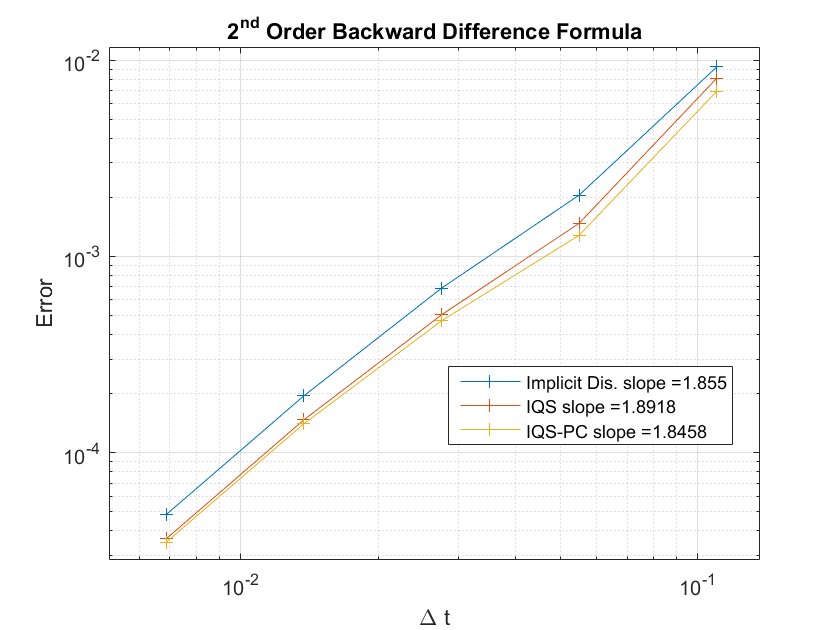
\includegraphics[width=\linewidth]{\FiguresDir/1D_conv_BDF2.png}
\caption{BDF2}
\end{subfigure}
\begin{subfigure}[b]{0.49\textwidth}
\centering
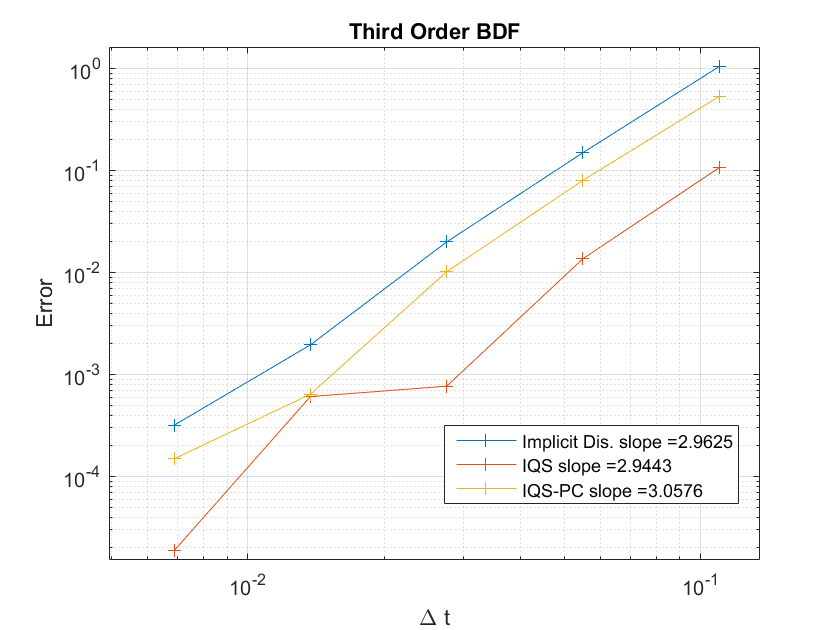
\includegraphics[width=\linewidth]{\FiguresDir/1D_conv_BDF3.png}
\caption{BDF3}
\end{subfigure}
\begin{subfigure}[b]{0.49\textwidth}
\centering
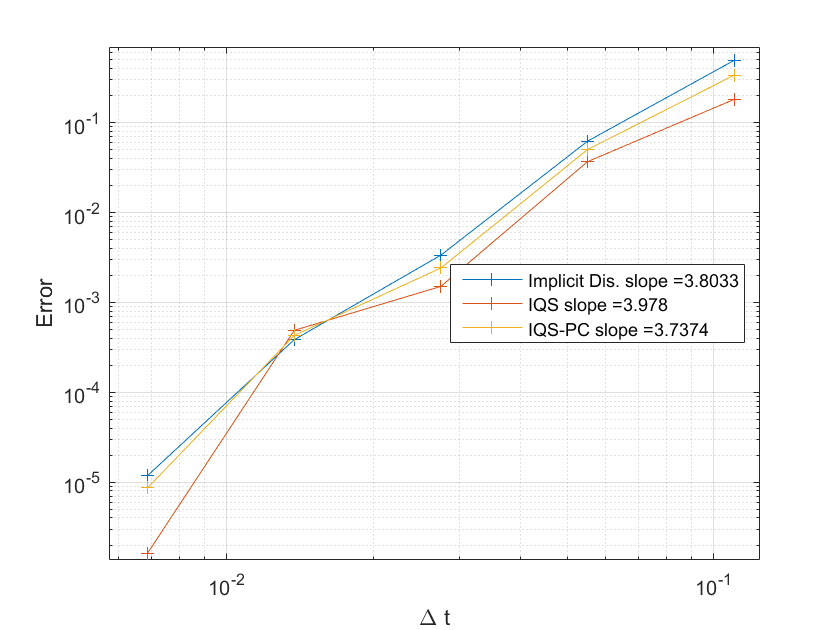
\includegraphics[width=\linewidth]{\FiguresDir/1D_conv_BDF4.png}
\caption{BDF4}
\end{subfigure}
\begin{subfigure}[b]{0.49\textwidth}
\centering
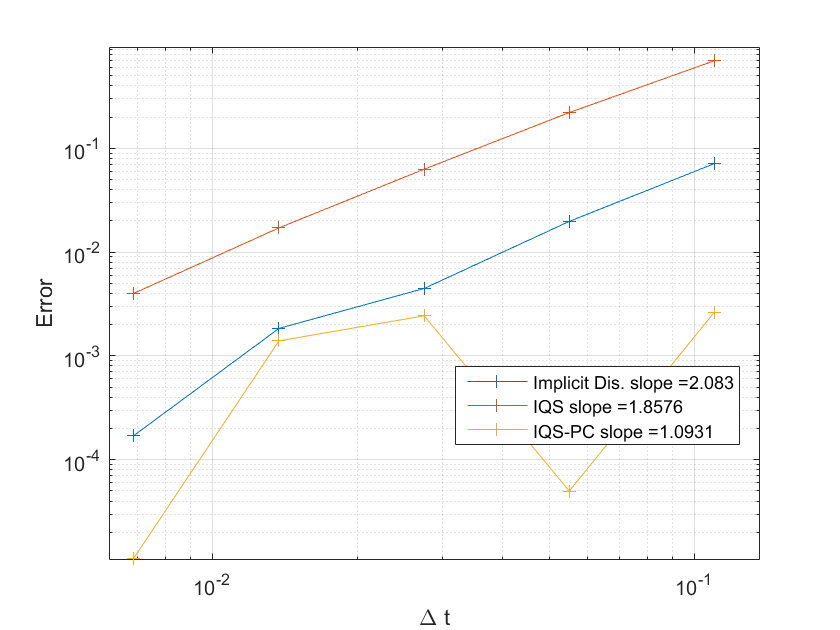
\includegraphics[width=\linewidth]{\FiguresDir/1D_conv_SDIRK33.png}
\caption{SDIRK33}
\end{subfigure}
\caption{Error convergence plots of implicit discretization, IQS, and IQS P-C with various time discretization schemes}
\label{fig:1D_conv}
\end{figure}

\begin{figure}[!htbp]
\begin{center}
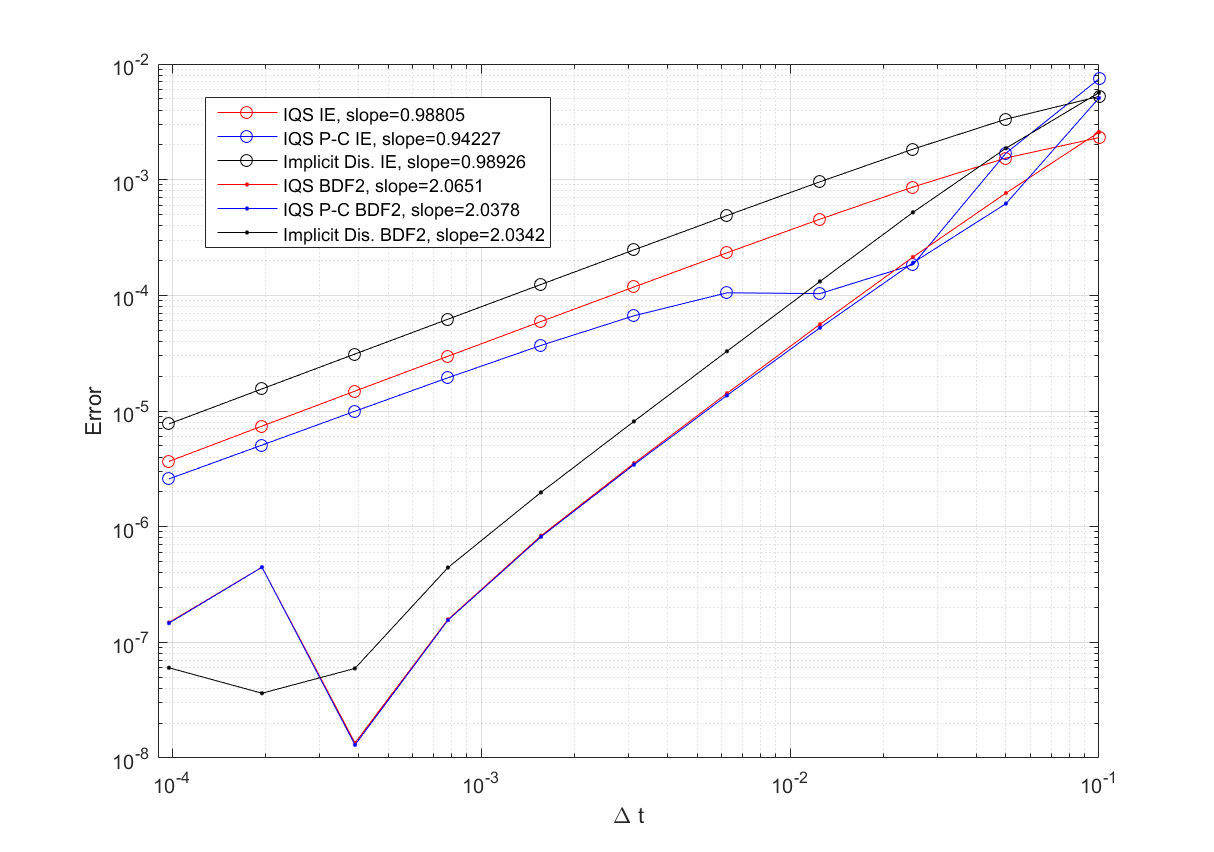
\includegraphics[width=0.75\linewidth]{\FiguresDir/1D_conv_Rat.png}
\caption{Error convergence plots of implicit discretization, IQS, and IQS P-C from Rattlesnake implementation}
\label{fig:1D_conv_Rat}
\end{center}
\end{figure}

\begin{figure}[!htbp]
\begin{center}
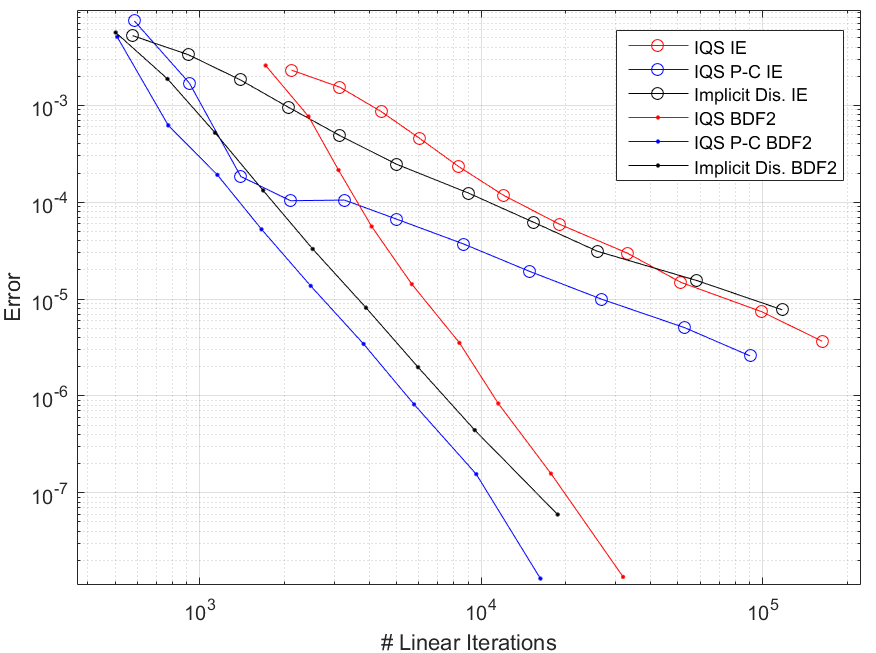
\includegraphics[width=0.75\linewidth]{\FiguresDir/1D_conv_lin.png}
\caption{Error convergence plots of implicit discretization, IQS, and IQS P-C vs. number of GMRES iterations}
\label{fig:1D_conv_lin}
\end{center}
\end{figure}

\pagebreak
\section{TWIGL Benchmark}

This benchmark problem originates from the Argonne National Lab Benchmark Problem Book \cite{ANL_BPB}.  It is a 2D, 2-group reactor core model with no reflector region shown in \fig{fig:TWIGL_reg} \cite{TWIGL_benchmark}.  This example is meant to be of progressive complexity from the previous example.  The transient of this reactor is very geometrically symmetrical with very little temporal shape change.  Therefore, IQS is expected to perform significantly better than the implicit discretization method.  \tbl{tab:TWIGL_mat} shows the material properties of each fuel region and the ramp perturbation of Material 1.

\begin{figure}[!htbp]
\begin{center}
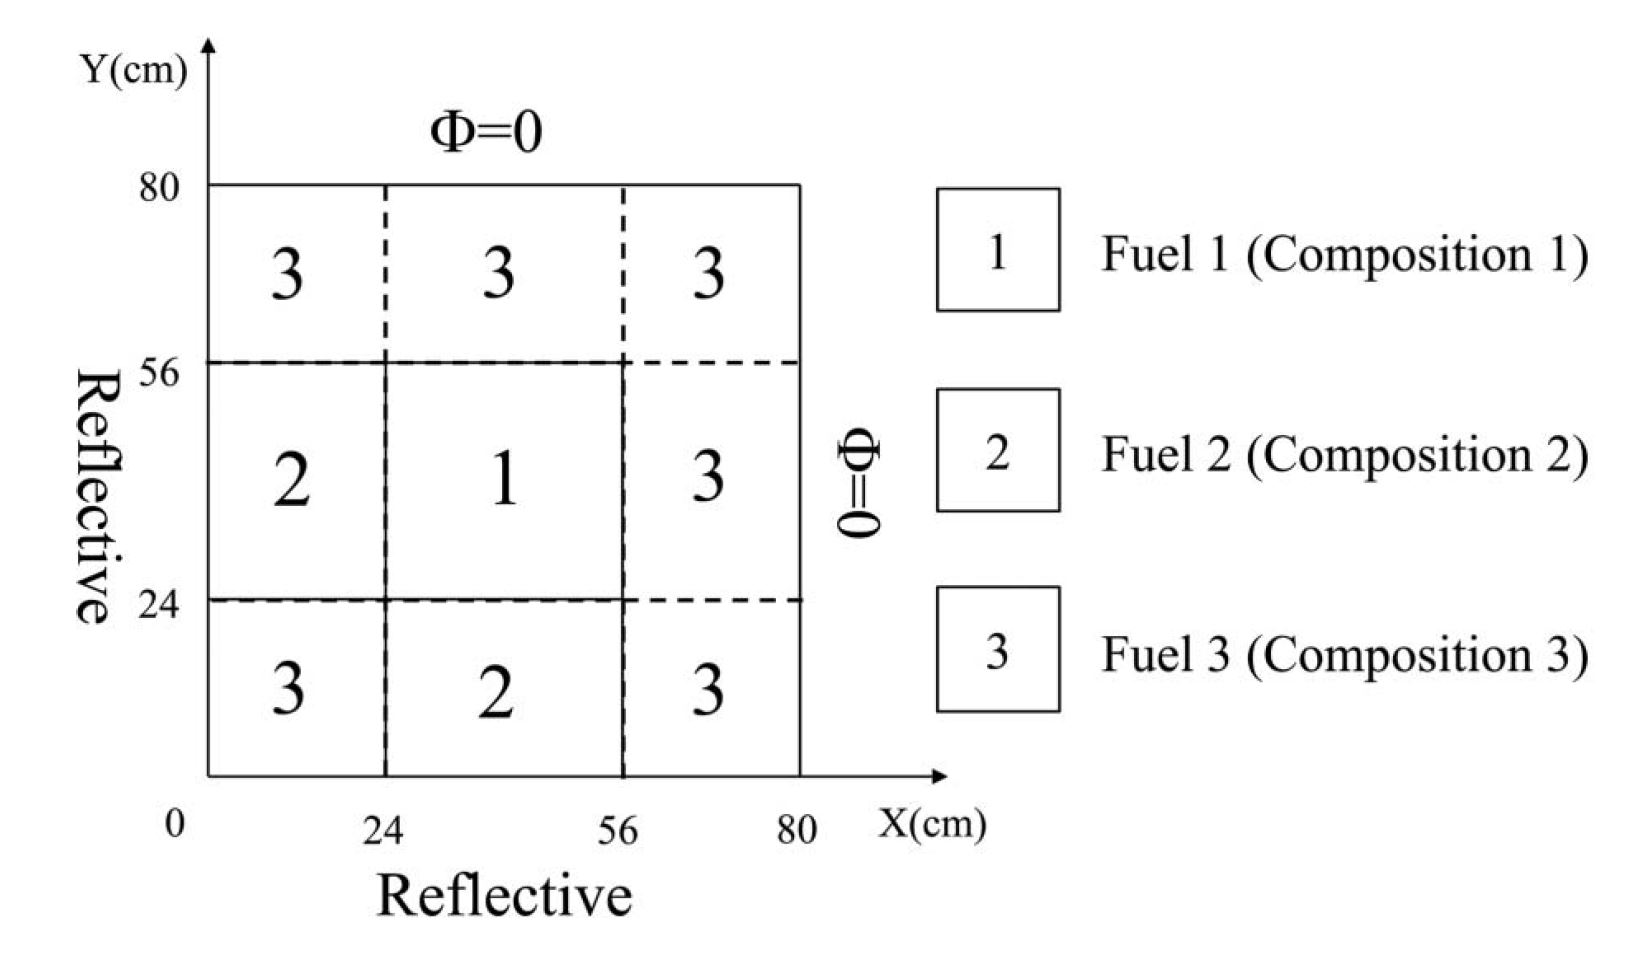
\includegraphics[width=0.75\textwidth]{\FiguresDir/TWIGL_regions.jpg}
\caption{TWIGL benchmark problem description}
\label{fig:TWIGL_reg}
\end{center}
\end{figure}
\begin{table}[!htbp]
\begin{center}
\caption{TWIGL benchmark material properties and slope perturbation}
\label{tab:TWIGL_mat}
\begin{tabular}{llllllll}
\hline
  &  &  &  &  &  &  \multicolumn{2}{c}{$\underline{\Sigma_s (cm^{-1})} $} \\
Material & Group & $D (cm)$ & $\Sigma_a (cm^{-1})$ & $\nu\Sigma_f (cm^{-1})$ & $\chi$ & $g \rightarrow 1$ & $g \rightarrow 2$ \\
\hline
1 & 1 & 1.4 & 0.010 & 0.007 & 1.0 & 0.0 & 0.01 \\
  & 2 & 0.4 & 0.150 & 0.200 & 0.0 & 0.0 & 0.00  \\
2 & 1 & 1.4 & 0.010 & 0.007 & 1.0 & 0.0 & 0.01  \\
  & 2 & 0.4 & 0.150 & 0.200 & 0.0 & 0.0 & 0.00  \\
3 & 1 & 1.3 & 0.008 & 0.003 & 1.0 & 0.0 & 0.01  \\
  & 2 & 0.5 & 0.050 & 0.060 & 0.0 & 0.0 & 0.00  \\
\hline
  & $\nu$ & $v_1 (cm/s)$ & $v_2 (cm/s)$ & $\beta$ & $\lambda (1/s)$ &   &   \\
\hline
  & 2.43 & 1.0E7 & 2.0E5 & 0.0075 & 0.08 &   &   \\
\hline
 \multicolumn{8}{l}{\footnotesize Material 1 ramp perturbation:} \\
\multicolumn{8}{l}{\footnotesize $\Sigma_{a,2}(t)=\Sigma_{a,2}(0) \times (1-0.11667t) \quad t \leq 0.2 s$} \\
\multicolumn{8}{l}{\footnotesize $\Sigma_{a,2}(t)=\Sigma_{a,2}(0) \times (0.97666t) \quad t > 0.2 s$} \normalsize
\end{tabular}
\end{center}
\end{table}

\subsection{TWIGL Convergence Analysis}


Figs. \ref{fig:TWIGL_power} and \ref{fig:TWIGL_plots} show the IQS  solution as compared with the implicit discretization solution.  It is important to note the IQS shape plot is scaled differently than the Brute Force flux plot (\fig{fig:TWIGL_plots}) because the amplitude term is not included, but the gradients of colors is comparable. These plots show that IQS is consistent in more complex, higher dimensional problems in Rattlesnake. These plots also serve to illustrate that IQS has a much more accurate solution, even at a significantly larger time step than the implicit discretization. In order to demonstrate asymptotic convergence of IQS, implicit Euler (IE) and second order BDF (BDF2) were applied to the TWIGL simulation. \fig{fig:TWIGL_conv} plots the error convergence of IQS and the implicit discretization methods.  The curves show the impressive convergence of IQS for the highly transient TWIGL example. The slope indicated in the legend are the linear slope of curves on the log plot, these slopes should be similar to the order of the method (1 for IE and 2 for BDF2).  IQS shows a increased order because the PRKE is performing much of accuracy convergence and it is computed using SDIRK33, a third order method.

\begin{figure}[!htbp]
\centering
\begin{subfigure}[!htbp]{0.49\textwidth}
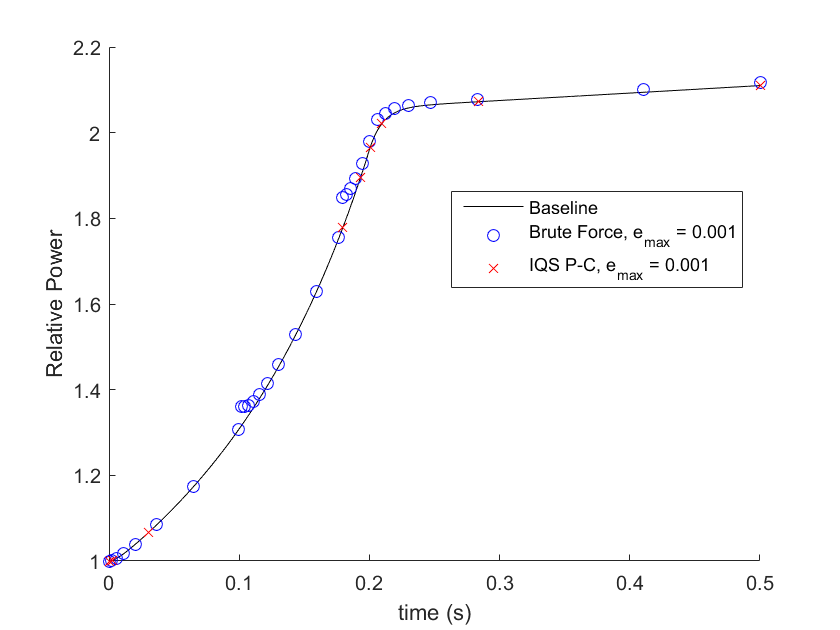
\includegraphics[width=\textwidth]{\FiguresDir/TWIGL_power_plot.png}
\caption{Power profile for entire transient}
\end{subfigure}
\begin{subfigure}[!htbp]{0.49\textwidth}
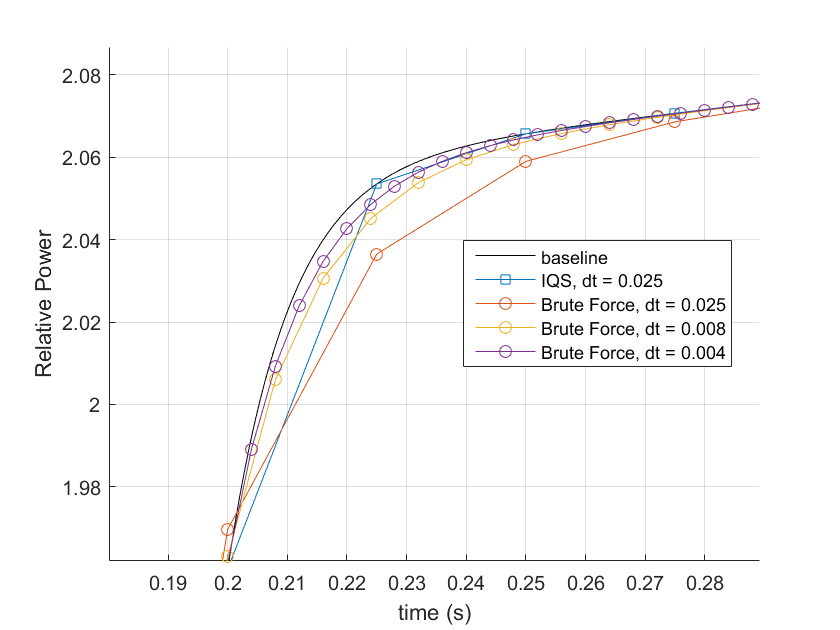
\includegraphics[width=\textwidth]{\FiguresDir/TWIGL_power_plot2.png}
\caption{Power at cusp of profile}
\end{subfigure}
\caption{Power level comparison of TWIGL Benchmark}
\label{fig:TWIGL_power}
\end{figure}

\begin{figure}[!htbp]
\begin{center}
\begin{subfigure}[!htbp]{0.4\textwidth}
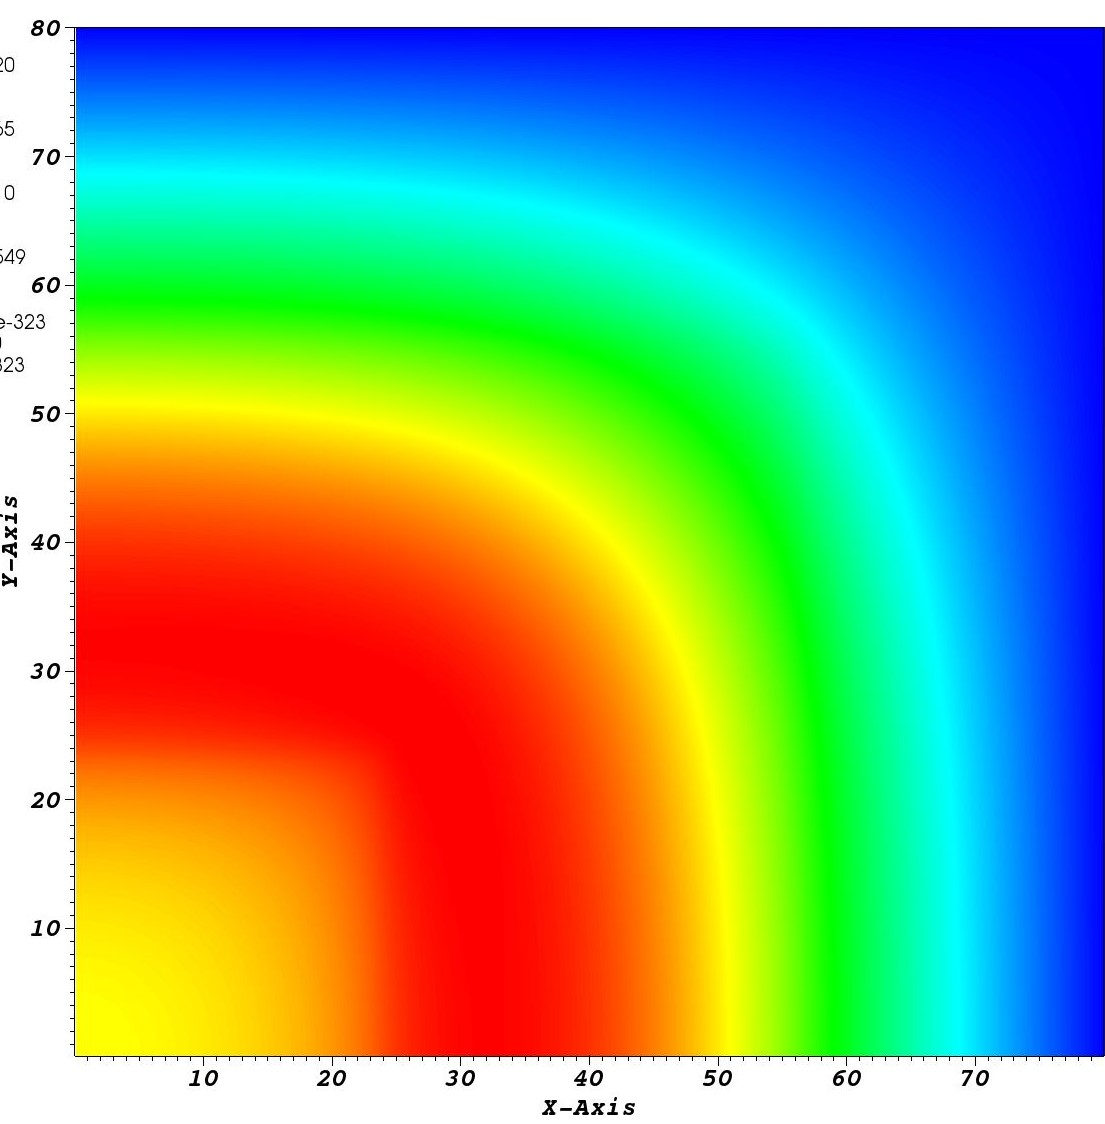
\includegraphics[width=\textwidth]{\FiguresDir/ndiff_ramp_flux.jpg}
\caption{Implicit Discretization flux}
\end{subfigure}
\quad
\begin{subfigure}[!htbp]{0.4\textwidth}
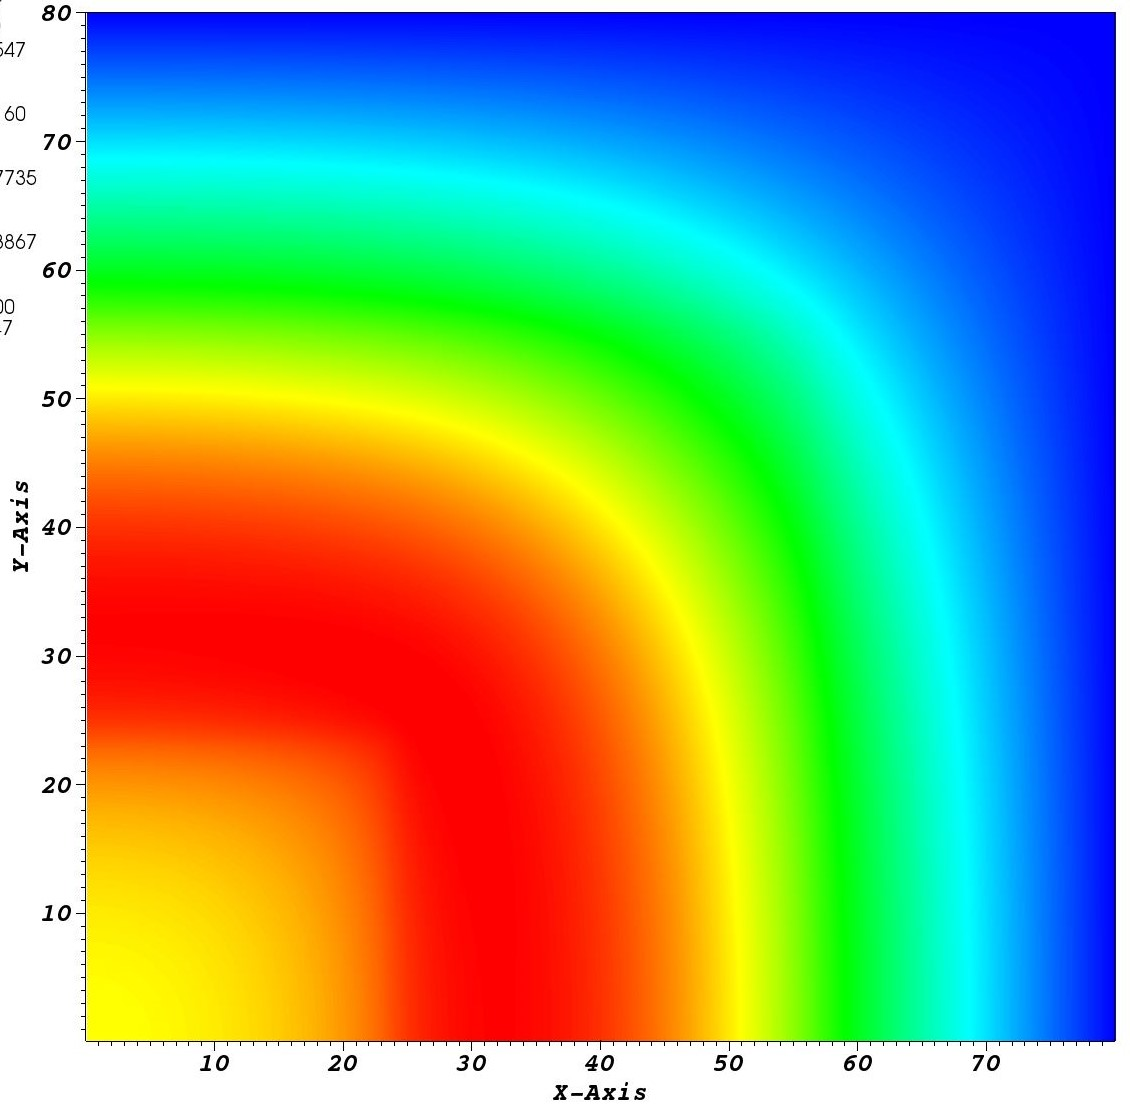
\includegraphics[width=\textwidth]{\FiguresDir/iqs_ramp_shape.jpg}
\caption{IQS Shape}
\end{subfigure}
\caption{TWIGL Benchmark flux/shape comparison at $t=0.2$}
\label{fig:TWIGL_plots}
\end{center}
\end{figure}

\begin{figure}[!htbp]
\centering
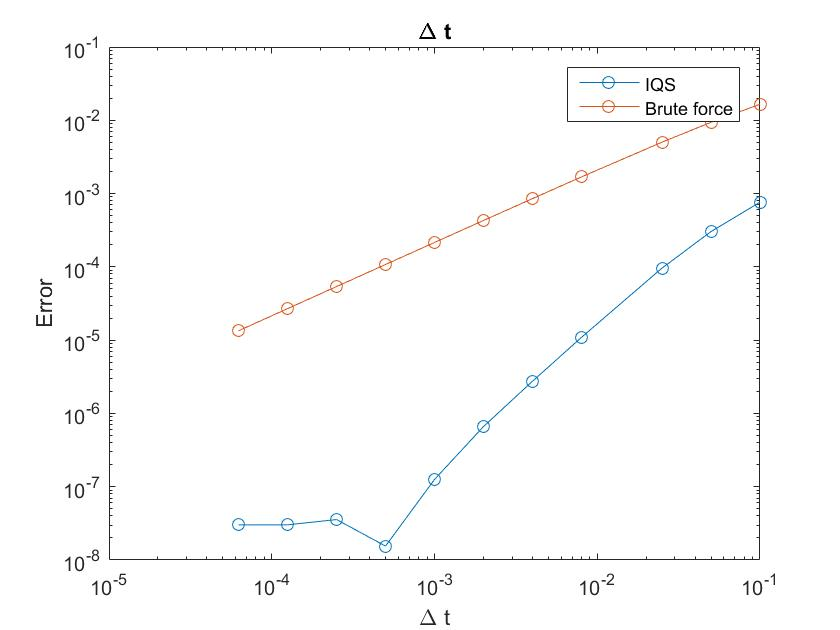
\includegraphics[height=3in]{\FiguresDir/TWIGL_convergence.jpg}
\caption{Error convergence comparison of TWIGL Benchmark}
\label{fig:TWIGL_conv}
\end{figure}

\subsection{TWIGL with Step Doubling Time Adaptation}

\tbl{tab:TWIGLdt2} and \fig{fig:TWIGL_power_dt2} show the results for TWIGL with time adaptation.  The results show that both IQS methods perform exceptionally well compared to implicit discretization.  It also shows that traditional IQS performed better with large $e_{tol}$, while IQS P-C was better with smaller $e_{tol}$.

\begin{table}[!htbp]
\begin{center}
\caption{TWIGL step doubling results}
\label{tab:TWIGLdt2}
\resizebox{\textwidth}{!}{
\begin{tabular}{|l|l|l|l|l|l|l|l|l|l|l|}
\hline
  &  & \multicolumn{3}{|c|}{Implicit Discretization} & \multicolumn{3}{|c|}{IQS} & \multicolumn{3}{|c|}{IQS P-C} \\
\hline
Test & $e_{tol}$ & Error & Steps & Solves & Error & Steps & Solves & Error & Steps & Solves \\
\hline
1 &	0.05    &	0.00012677 &	9   &	29  &	0.03380433 &	4   &	20   &	0.00323100 &	4  &	9   \\
2 &	0.01    &	3.5555e-05 &	11  &	35  &	0.00166991 &	5   &	40   &	0.00263068 &	5  &	12  \\
3 &	0.005   &	4.0364e-05 &	11  &	31  &	0.00886584 &	5   &	40   &	0.00160486 &	6  &	21  \\
4 &	0.001   &	0.00294822 &	33  &	122 &	0.02976305 &	5   &	36   &	1.7527e-05 &	10 &	35  \\
5 &	0.0005  &	0.00099778 &	39  &	131 &	0.00143781 &	6   &	55   &	1.4185e-05 &	16 &	74  \\
6 &	0.0001  &	0.00019510 &	78  &	236 &	0.00016175 &	8   &	65   &	6.2903e-06 &	19 &	78  \\
7 &	5.0e-05 &	0.00018372 &	112 &	342 &	6.0328e-05 &	12  &	163  &	1.5247e-06 &	24 &	92  \\
8 &	1.0e-05 &	8.0564e-05 &	263 &	794 &	7.7103e-05 &	379 &	5729 &	9.8321e-07 &	48 &	210 \\
\hline

\end{tabular}}
\end{center}
\end{table}

\begin{figure}[!htbp]
\centering
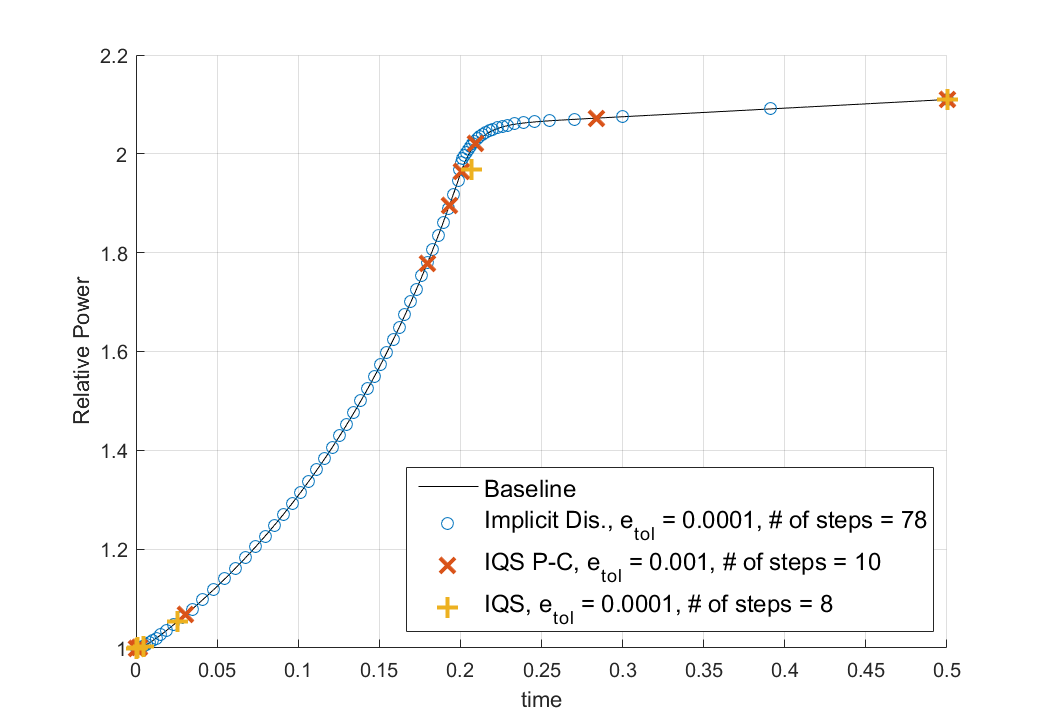
\includegraphics[width=0.8\linewidth]{\FiguresDir/TWIGL_power_plot_dt2.png}
\caption{Power level comparison of TWIGL Benchmark with time adaptation}
\label{fig:TWIGL_power_dt2}
\end{figure}

%\pagebreak
%\section{C5G7-TD Benchmark}
%
%The C5G7 benchmark is a MOX fueled, pressurized water reactor (PWR) minicore configuration. The C5G7 geometry depicted in Fig. \ref{fig:c5g7-2D} comprises a 2-by-2 array of UO$_2$ and MOX assemblies surrounded by moderator. In Fig. \ref{fig:c5g7-2D} vacuum and reflective boundary conditions are denoted by V and R, respectively. The fuel pins are not homogenized, each pin cell is comprised of a fuel pin, fission chamber, or guide tube surrounded by moderator as depicted in Fig. \ref{fig:c5g7-pincell}. The cladding and gap are homogenized into the fuel and are not explicitly modeled. Each assembly is made up of a regular 17-by-17 grid of pin cells.
%Seven energy-group cross sections for the seven material regions are given in \cite{c5g7}. The energy group boundaries are provided in Table \ref{tab:c5g7-ebounds}; three of the seven energy groups are fast, four are thermal.
%
%\begin{figure}[!htpb]
%\begin{center}
%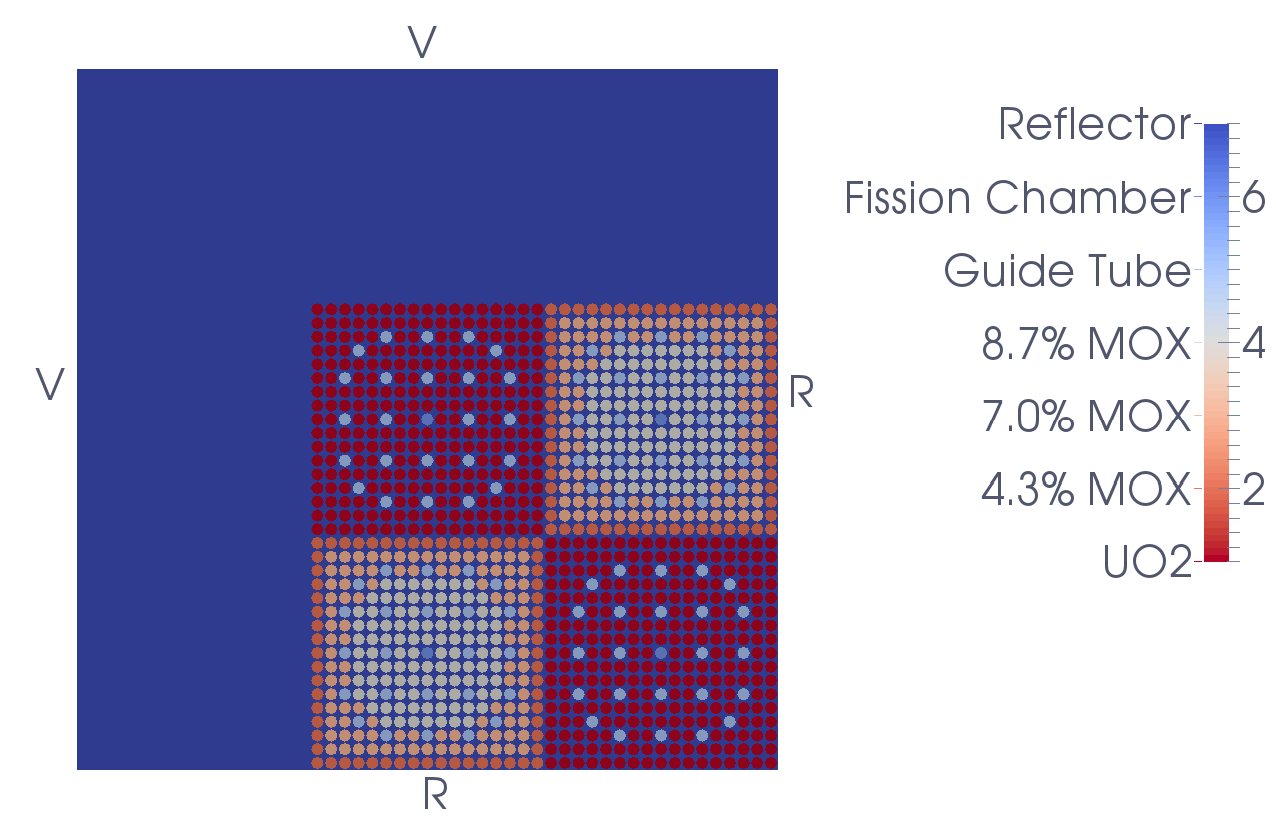
\includegraphics[width=\linewidth]{\FiguresDir/C5G7-2D.png}
%\end{center}
%\caption{Geometry of the two-dimensional C5G7 benchmark problem. Boundary conditions are vacuum (V) or reflective (R).}
%\label{fig:c5g7-2D}
%\end{figure}
%
%\begin{figure}[!htpb]
%\begin{center}
%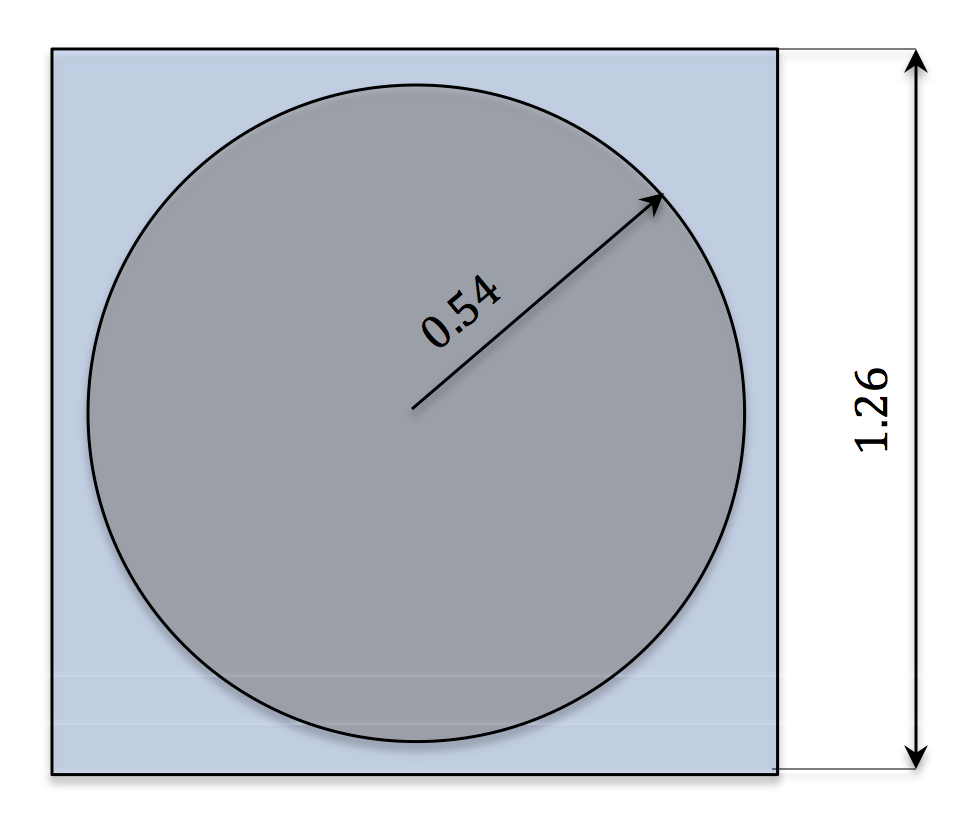
\includegraphics[width=0.5\linewidth]{\FiguresDir/C5G7-pincell.png}
%\end{center}
%\caption{Geometry of a C5G7 pin-cell.}
%\label{fig:c5g7-pincell}
%\end{figure}
%
%\begin{table}[!htpb]
%\centering
%\caption{Energy group boundaries for C5G7 MOX benchmark.}
%\label{tab:c5g7-ebounds}
%\begin{tabular}{c c}
%\hline
%Group & Upper Energy\\
%\hline
% 1&20 MeV  \\
% 2&1 MeV  \\
% 3&500 keV  \\
% 4&3 eV  \\
% 5&0.625 MeV  \\
% 6&0.1 MeV  \\
%71&0.02 MeV  \\
%\hline
%\end{tabular}
%\end{table}
%
%\pagebreak
%\section{LMW Benchmark?}

